
%What is eels?
%Sample experimental setup
%Sample spectra
%Signal types
%usages
%pros, cons/ STEM TEM
\setcitestyle{numbers,open={[},close={]}}

 


Many of the results from EELS have non-intuitive interpretations, particularly in the case of ELNES which relies primarily on qualitative comparisons between measured and database spectra.  Consequently, new materials require theoretical support to analyze results.  This support often comes from \textit{ab initio} calculations, such as density functional theory (DFT).  This section  describes the basis of DFT and its various implementations, as well as the peculiarities of simulating lithium materials.

\subsection{DFT Background}
DFT is an \textit{ab initio} method that requires only atomic positions as input and is independent of experimental support.  By solving a modified version of the Schrodinger equation, it is possible to obtain the ground state energy of the system, and from there determine a range of  properties, including EELS spectra. This almost direct treatment of quantum mechanics makes DFT one of the most accurate techniques of first principle simulations. However, the quadratic to cubic scaling of the method with the number of electrons, limits its applicability to small scale systems, typical size limitations shown in Fig \ref{scaling}.  DFT's accuracy and flexibility have resulted in the development of a large number (90+) of codes, both open source and commercial \cite{DFT_codes}.  

\begin{figure}
	\centering
	\includegraphics[width=0.5\textwidth]{method_scaling.png}
	\caption{Various methods available to compute material properties and their corresponding regions of use. }
	\label{scaling}
\end{figure}


\subsection{Formulation}

DFT is centred  on solving the many bodied  Schrodinger equation \cite{sholl_density_2009}.  The quantity in question is a solution for $\psi_i$, the electron wavefunctions from which observable properties can be calculated:  

\begin{equation}
	\frac{-\hbar^2}{2} \sum_{i}^{N} \frac{\nabla^2 \psi_i}{m_i} + \sum_{i}^{N} V(\textbf{r}_i) \psi_i = E \psi
\end{equation}

In this case, the non-relativistic, spin independent, time independent case is considered, although more in-depth derivations can be found elsewhere \cite{tddft}. The Born Oppenheimer approximation is now applied, which assumes that the nuclei can be separated from the electrons and will act classically. The validity of this assumption stems from the fact that nuclei are over 1000 times more massive than electrons \cite{graff_direct_1980}.  Applying the Born Oppenheimer approximation results in only needing to solve for the $\psi$ of electrons and allows the potential to be broken up:

\begin{equation}
	\bigg[\frac{-\hbar^2}{2m_e}\sum_{i}^{N} \nabla^2 +\sum_{i}^{N} V(\textbf{r}_i) + \sum_{i}^{N}\sum_{j <i}U(\textbf{r}_i,\textbf{r}_j) \bigg] \psi_i(\textbf{r}_i) = E \psi_i
\end{equation}

Where $m_e$ is the mass of an electron, $N$ is the number of electrons, and $\textbf{r}_i$ is a position vector. The terms inside the square brackets are collectively known as the Hamiltonian and are respectively: the kinetic energy of all the electrons, the Coulomb interaction between the electrons and the nuclei, and the electron-electron Coulomb interaction  \cite{sholl_density_2009}. At this point, the equations are still too unwieldy to solve, depending on 3N variables (the position coordinates of each wavefunction), not to mention the many body problem lurking inside the double sum.  Facing this conundrum, the Hohenberg-Kohn Theorems are applied which postulate that \cite{hohenberg_inhomogeneous_1964}:
\begin{itemize}
	\item  The ground state \textit{energy} of the system is a unique functional of the ground state \textit{electron density}.
	\item The electron density which minimizes the overall energy corresponds to the real ground state electron density.  
\end{itemize}

By changing the variables being solved for to the \textit{density} and not wavefunctions, the problem is reduced down to only three variables: the three coordinates of the density field.  The Hohenberg-Kohn theorems indicate that the observables can all be made into functionals of electron density and that any density other than the groundstate will result in a higher energy in the system \cite{parr_density_1983}.  The term functional is defined as an object that acts similar to a function, except that it takes other functions as input instead of variables, eg:

\begin{equation}
F[f(x)] = \int f(x) dx
\end{equation}

 In DFT, the relevant functional is the energy which is a functional of the density: $E[n(\textbf{r})]$.  Using the Hohenberg-Kohn theorems, it is possible to work towards a more manageable equation for energy as a functional of density by breaking down the potentials: 
\begin{equation}
-\frac{\hbar}{2m_e} \sum_{i} \int \psi_i^* \nabla^2\psi_id^3r + \int V(\textbf{r})n(\textbf{r})d^3r + \frac{e^2}{2} \int \int \frac{n(\textbf{r})n(\textbf{r}')}{|r-r'|}d^3r d^3r' + E_{\mathrm{nuclei}} + E_{\mathrm{XC}} = E[n(\textbf{r})]
\end{equation}

Where the second term is the energy from the electron density-nuclei interaction, the third term is the electron density-electron density Coulomb interaction and $E_{\mathrm{nuclei}}$ is the contribution from nucleus-nucleus interaction.  The final term, $E_{XC}$ is the exchange and correlation term, where all of the quantum features of the electrons are grouped the result of basing the analysis in terms of density. This equation cannot be directly solved from first principles by itself as a means is needed to obtain the electron density.  On this front, the Kohn -Sham equations are introduced, which assume that the electrons can be decoupled into single particle equations: 

\begin{equation}
    \bigg[T_i + V(\textbf{r}) + V_{\mathrm{H}}(\textbf{r}) + V_{\mathrm{XC}}(\textbf{r})\bigg] \phi_i(\textbf{r}) = \epsilon_i \phi_i(\textbf{r})
    \label{ks_eq}
\end{equation}

Where $\phi_i$ and $\epsilon_i$ are the Kohn sham wavefunctions and eigenvalues respectively and $V_H$ is the Hartree potential or: 
\begin{equation}
    V_\mathrm{H} = e^2 \int \frac{n(\textbf{r'})}{|\textbf{r}-\textbf{r'}|}d^3r'
\end{equation}
The Hartree potential represents the interaction of the electron in question (the one at $\textbf{r}$, not $\textbf{r'}$) and all the electrons in the sample.  This results in some interaction between the electron and itself, a term that must be corrected for in the $V_{XC}$ term.  The Kohn-Sham equations can  be readily solved, but require the density to calculate the Hartree potential.  The density is in turn obtained from the wavefunctions: 
\begin{equation}
	n_{\mathrm{KS}}(\textbf{r}) = 2 \sum_{i} \phi_i^*\phi_i
	\label{KS_density}
\end{equation}
Where the factor of two is to account for electron spin.  As the density is needed to calculate the wavefunctions and vice versa, a self consistent approach must be taken in order to obtain a valid result:  

\begin{enumerate}
	\item Assume a starting density
	\item Use the initial density to calculate the Hartree potential and use it to solve the Kohn-Sham equations for the wavefunctions
	\item Calculate a new density using Eq. \ref{KS_density}.
	\item Compare the new density to the initial and update the initial density. 
	\item Repeat steps 2-4 until the density converges and the energy is minimized. This density then represents the groundstate for the system.
\end{enumerate}

This method is the starting point for DFT calculations, from which there are a number of  variations with regarding how to proceed with these steps.  Amongst these, the treatment of the exchange-correlation potential and choice of basis for the wavefunctions separate the various methods common in DFT packages.  


\subsubsection{Exchange-Correlation Potential}
The exchange-correlation potential was introduced above, but not explicitly defined.  That is because there no easily solvable form, for this term as it collects all of the unknown attributes not accounted for in the Kohn-Sham equations.  These include accounting for electron's being indistinguishable, the self interaction term, etc.   There have been a number of proposed potentials, many designed for specific situations the most common of which will be discussed here.  Like the potentials in the Kohn-Sham equations, the XC potential is defined as a functional of density.  The various potentials vary according to accuracy and computational cost.  The first attempt, originally proposed by Kohn and Sham in 1965 was the local density approximation (LDA) in which the exchange and correlation potential depends only on the density \cite{tao_climbing_2003, ks_1965}: 

\begin{equation}
	E_{\mathrm{XC}}[n(\textbf{r})] = \int  n(\textbf{r}) \epsilon_{\mathrm{XC}}[n(\textbf{r})] d^3r
\end{equation}

LDA is exact in the case of a free electron gas and has obtained good success when applied to metallic solids.  By also considering the gradient of the density, a more involved potential is obtained, called the generalized gradient approximation (GGA) \cite{tao_climbing_2003,perdew_wang} : 


\begin{equation}
E_{\mathrm{XC}}[n(\textbf{r})] = \int  n(\textbf{r}) \epsilon_{\mathrm{XC}}[n(\textbf{r}), \nabla n[\textbf{r}]] d^3r
\end{equation}


Other parameters can also be taken into consideration, such as the potential energy (meta GGA), empirical factors, or mixing with the exact Hartree-Fock (hybrid functionals) \cite{tao_climbing_2003, bj_pot}.  Depending on the desired property and available computing power, an appropriate functional must be chosen for each case.


\subsubsection{Basis Sets}
A second defining feature for various DFT methods is the choice of basis set for the wavefunctions, $\phi_i$.   A number of options have become prevalent in the available programs.  These are divided into two distinct types, localized and periodic \cite{sholl_density_2009}.  Localized basis sets rely on using orthogonal functions which decay rapidly away from the origin \cite{sholl_density_2009}.  An example is Gaussian peaks, as is used in the Gaussian16 software package \cite{g16}.  The very localized basis set is useful for handling single, isolated molecules, which is ideally suited applications in quantum chemistry and biology. Poor scaling with electron number (typically N$^3$ or worse) limits the maximal size of system that can be studied \cite{mohr_linear_2018}.  In materials science, a typical system of interest is a bulk material and thus unsuitable for this approach.  To handle these cases, periodic basis sets are used, by defining a unit cell and repeating it infinitely in all directions.  The solution to the Schr\"odinger equation under these periodic boundary conditions is given by Bloch waves, defined as \cite{griffiths}:

\begin{equation}
	\psi = u(\textbf{r}) e^{i\cdot \textbf{k}}
\end{equation}

Consequently, a natural basis choice for periodic boundary situations are plane waves, which are used in a number of DFT packages including VASP, Quantum Espresso, and WIEN2k \cite{qe,vasp,wien2k}.  The periodic boundary method allows for accurate calculation of in infinite samples, representative of bulk materials.  The computational limits then apply to the size of the unit cell, typically limited to at most a few hundred atoms \cite{mohr_linear_2018}.  These limits render features such as defects and grain boundaries computationally expensive as they must be contained in a cell large enough to isolate them from their repeated images in adjacent cells. 
As large numbers of plane waves would be required to handle the fine features in the electron density close to nuclei, often an augmented plane wave (APW) technique is used.  APW lowers the computational cost by dividing the unit cell into two regions: interstitial space and atomic basins (sometimes referred to as muffin tins), illustrated  in Fig \ref{MT} \cite{wien2k}. \\
\begin{figure}
	\centering
	\includegraphics[width=0.5\textwidth]{muffin_tins.png}
	\caption{The two regions in an augmented plane wave approach.  (I) Atomic Basins modelled with Psudopotentials or atomic orbitals and (II) interstitial space modelled with a plane wave basis set.  Taken from Schwarz, 2002 \cite{wien2k}. }
	\label{MT}   
\end{figure}

The ability to divide electrons into two groups is valid as the core electrons surrounding each atom are largely isolated from the local environment by the outer shells \cite{wien2k}. The choice of which basis set is used inside the muffin tins provides additional options distinguishing DFT codes.  One option is pseudopotentials, which are pre-generated densities for each element and can be varied to match the plane waves at the boundary \cite{singh_planewaves_2006}.  The pseudopotential method is used in programs such as VASP and Quantum Espresso \cite{vasp,qe}.  Alternatively, spherical harmonics corresponding to the atomic orbitals can be used for increased accuracy \cite{griffiths}. This type of DFT is referred to as all-electron or full potential, as every electron is represented in the basis set, unlike the pseudopotential method where core electrons are absorbed into the pre-calculated pseudopotential \cite{wien2k}. Fitting for all of the electrons in the sample comes at a computational cost, yet allows for more a accurate analysis of the properties dependent on core states, such as ELNES spectra in EELS.   \\
 
 A flowchart demonstrating the various properties of some common DFT codes is illustrated in Fig \ref{dft-flowchart}.  The DFT code used primarily in this work is WIEN2k and is presented in the following section.

\begin{figure}
	\centering
	\includegraphics[scale=0.3]{DFT_flowchart.png}
	\caption{Flowchart depicting the various choices of basis set available to DFT codes.}
	\label{dft-flowchart}
\end{figure}


\subsection{WIEN2k}
WIEN2k is an all electron code that uses a linearized augmented plane wave (LAPW) formulation, combining plane waves with spherical harmonics illustrated in Fig \ref{MT} \cite{wien2k}.   In WIEN2k's standard formalism, the basis sets for the Kohn-Sham wavefunctions can be represented as: 

\begin{equation}
	\phi_{\mathrm{k}_n} = 
	\begin{cases}
	\Sigma_{lm} [A_{lm,\textbf{k}_n}u_l(r,E_l) + B_{lm,\textbf{k}_n}\dot{u}_l(r,E_l)]Y_{lm}(\hat{\textbf{r}}) & r \leq r_{\mathrm{RMT}} \\
	\frac{1}{\sqrt{\omega}}e^{i\textbf{k}_n \cdot \textbf{r}} & r> r_{\mathrm{RMT}} \\
	\end{cases}
\end{equation}

Where \textit{n, l}, and \textit{m} are the principle, azimuthal and magnetic quantum numbers respectively, $Y_{lm}(\hat{\textbf{r}})$ are the spherical harmonics and $u_l(r,E_l)$ are the solutions to the radial Schr\"odinger equation.  The coefficients $A_{lm,\textbf{k}_n}$ and $B_{lm,\textbf{k}_n}$ are set to match the value and slope of the plane waves at the boundary \cite{wien2k}.  The use of an all electron code is essential for computing EELS accurately as it allows for a more flexible treatment of the core electrons not granted in pseudopotential codes. 
 


\subsection{Quantum Theory of Atoms in Molecules} \label{bader-theory}
Before continuing to the application of DFT to EELS,  a more direct application of DFT is briefly presented: defining atoms and bonds from the electron density. Initial work on this front was performed by Bader, resulting in the field sometimes being referred to as Bader Theory \cite{bader}. The electron density can be divided into regions, with each atomic basin  delimited by surfaces satisfying \cite{bader_quantum_1991}: 


\begin{equation}
\nabla \rho(\textbf{r}) \cdot \textbf{n}(\textbf{r}) = 0   \hspace{1cm} \forall\textbf{r} \in S(\Omega,\textbf{r})
\label{basin_surface}
\end{equation}

That is, surfaces with no flux of electron density through them which can be pictured as a ``valleys" in the electron density ``landscape," see Fig \ref{topo_plot}. In order to  rapidly calculate the location of these surfaces, critical points in the density field are located, satisfying $\nabla \rho(\textbf{r})=0$.  These critical points will always satisfy Eq. \ref{basin_surface}.  With the exception of critical points at maximas in $\rho(\textbf{r})$ which are located at nuclei, all of the critical points lie on interatomic surfaces \cite{critic2}. The nature of the critical points can then be evaluated (minima, first or second order saddle point), and the location of bonds which are centred on first order saddle point critical points, can be determined \cite{critic2}.  The bonds can then be characterized to provide first principles chemical bonding analysis for quantum chemistry \cite{fugel_variety_2018}.  

\begin{figure}
	\centering
	\includegraphics[width=0.75\textwidth]{bader_topo_plot}
	\caption{Density plot (left) and identification of atomic basin (right) in a diborane molecule. From Bader, 1998 \cite{bader}.}
	\label{topo_plot}
\end{figure}


\subsection{Lithium in DFT}
Lithium's low atomic number requires a number of special treatments  in DFT.  These are mainly due to its loosely bound electrons with large orbitals resulting from lithium's small nuclear charge.  Even the 1s level electrons in lithium can have orbitals extending well past 2.5 Bohr from the nuclei, far further than in heavier elements, see Fig \ref{orbital_size} where a range of orbital sizes are compared \cite{mauchamp_ab_2006}.  This results in a number of issues. One of these is that it is difficult and sometimes impossible to set the atomic sphere radii large enough to contain all these 1s core electrons.  As atomic spheres cannot overlap, they are typically limited to $\sim$ 2.0 Bohr. Depending on the compound, the sphere size can be further constrained as all the spheres must be roughly the same size (within 30\%) \cite{wien2k}.  If the sphere sizes are too varied, convergence time and accuracy can deteriorate dramatically.  The alternative to large sphere size is to allow a degree ($\sim$0.5\%)of core leakage into the calculation \cite{wien2k}.  The downside to allowing leakage is that it may result in non physical effects at later stages in the calculation, or in the appearance of ``ghostbands" in the calculation \cite{wien2k}.

\begin{figure}
	\centering
	\includegraphics[width=0.75\textwidth]{atomic_orbital_size}
	\caption{Orbital charge densities as a function of distance from nucleus, demonstrating the varying degrees of localization.  From Mauchamp \textit{et al}, 2006 \cite{mauchamp_ab_2006}}
	\label{orbital_size}
\end{figure}



